\subsection{Story: Admins can login to the backend and run a session with a quiz}
\subsubsection{Analysis - breakdown of tasks}
Tasks left over from the previous week:
\begin{itemize}
	\item Form on front page redirects to quiz
	\item Questions rendered as a form
	\item User can submit the form with their answers
	\item Questions need limiting on going above/ below max and min
\end{itemize}
\subsubsection{Design}
The only new design for this story from the last iteration is to add to the use case for students on the frontend. \ref{fig:iter-5-frontend-use-case}

\begin{figure}
	\caption{Use case for front end now including what students can do}
	\centerline{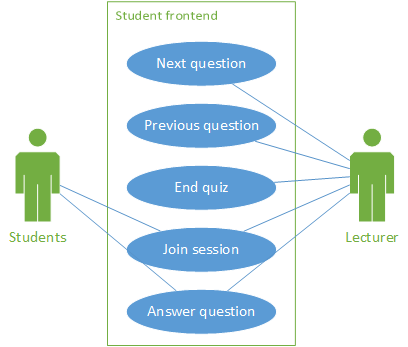
\includegraphics{Chapter2/Iter-5/iter-5-frontend-use-case}}
	\label{fig:iter-5-frontend-use-case}
\end{figure}

\subsubsection{Implementation}
Users still had to connect to the quizzes from the welcome page. A problem with this is that the sessions are being run under the url /quiz/session\_name. This means that submitting a GET or POST form will not work as the url cannot be specified, as the user enters the session key. A solution was to have an input field that took the session key and then used JavaScript to redirect to that session. An alternative solution would be to use a form that redirected to a controller action that then itself redirected to the correct session page. Whilst this method would work, having multiple redirections in one request is not good practice or nice for the users browser.

The JavaScript also allowed some client side checking to be done, but there also needed to be server side checks. A custom Middleware class was written to handle the checking of valid session keys. Middleware provides the functionality to filter incoming HTTP requests within controllers\cite{laravel-middleware}. When the form was submitted, the Middleware function would check the database, and if the requested key was not in the database, would redirect back to the welcome page with an error. Else, it would allow the redirection to the quiz session.

When the page receives a message through the Web Sockets, it first removes the content of the page with JQuery. It then checks the position of the quiz, if it is zero, then it appends the quiz start data on to the page. This start data includes information about the quiz, like the name and description. If the position is not zero, then it will render the question at that position in the quiz.

To render a question, an Ajax request is made to a question page that will be populated with the appropriate data using the information from the Web Sockets as the variables for finding the correct question. The Ajax'ed page content is then appended on to the current page using more JQuery.

For the user to submit an answer, the form again had to use JavaScript. This was primarily to make the form user friendly and for different questions types. JS was used to add a class to the options and highlight the ones that were chosen, be it one option in a multiple choice question or multiple answers on a multiple selection question. When the student hits submit, it gets the answers by selecting the options with the classes that are added when an option is selected. It then sends a POST request with Ajax to the quiz session page. The POST'ed data consisted of the answers given, in the form "answer*" where the * was the answer number as well as the question number. This data is not yet handled by the server.

A bug with multiple selection questions was with the answers selection. To get just the answer value, the array of elements was iterated over and a new array with the answers is produced. However, due to using a JQuery array function to iterate over these, it created a JQuery collection, rather than a simple array. This collection was not accepted by the Ajax request and this collection has to be transformed into an array with a vanilla JS toArray() function.

The last part of development for this iteration involved adding some simple checks to the next and previous position functions to ensure they did not go below 0 or above the number of questions in the quiz.

\subsubsection{Testing}
A number of tests were written for this large part of the system split into three main areas: admins running quizzes, students joining quizzes, and multiple sessions being run simulataneously. Some of tests used Dusks ability to create two browsers and imitate two users of the system, this was used to check WebSocket functionality. TODO: explain problems here?
\newpage

\subsection{Non-story work}
\subsubsection{User page}
Significant work was done on the user pages, this was to ensure that an admin could view and edit their details including changing their session keys. This work was rather simple and just involved creating the user blade pages, adding the various functions to the controller and model and adding a little bit of functionality to the authentication actions for registering a new user. Very similar work took several hours when the initial quiz pages were created, however with the experience from that work this only took an hour. Figure \ref{fig:iter-5-users-use-case}

\begin{figure}
	\caption{Use case for the users page}
	\centerline{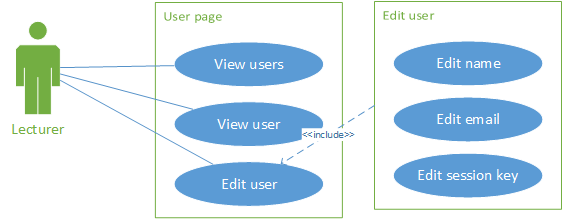
\includegraphics{Chapter2/Iter-5/iter-5-users-use-case}}
	\label{fig:iter-5-users-use-case}
\end{figure}

\subsubsection{JavaScript clean up}
A lot of JavaScript that was being rendered on the page is not used and useless to the project, in fact the libraries are quite large and take up a significant amount of space. Removing these unused libraries, VueJs being the largest, frees up the JavaScript output file considerably, which will increase load times significantly.
\newpage
